% \cite{palomar:portfolio_optimization}
so far assumed: parameters of the state space models are known and only the state needs to be estimated. In practical models, the parameters are unknown as well. In this chapter, there are three types of methods for parameter estimation. 
\begin{enumerate}
    \item Optimization-based methods for computing maximum a posteriori (MAP) or maximum likelihood (ML) estimates
    \item Expectation-maximization (EM) algorithms for computing the MAP or ML estimates
    \item Markov chain Monte Carlo (MCMC) methods for generating Monte Carlo approximations of the posterior distributions
\end{enumerate}
% Bayesian Estimation of Parameters in State Space Models
% Parameter Posterior and Energy Function
% Maximum A Posteriori and Laplace Approximations
% State Augmentation Approach
% Parameter Estimation in Linear State Space Models
\begin{theorem}[Energy function for linear Gaussian model]
    The recursion for the energy function is given as 
    \[\psi_k(\theta) = \psi_{k-1} + \frac{1}{2}log\textbf{ }|2\pi\textbf{ 
    }\mathbf{S}_k(\theta)| + \frac{1}{2}\mathbf{v}_k^\intercal(\theta)\textbf{ }\mathbf{S}_k^{-1}(\theta)\mathbf{v}_k(\theta), \]

    where the terms $\mathbf{v}_k$ and $\mathbf{S}_k(\theta)$ are given by the Kalman filter with the parameters fixed to $\theta$.
    \begin{itemize}
        \item Prediction: 
            \begin{itemize}
                \item[] $\mathbf{m}_k^-(\theta) = \mathbf{A}(\theta)\textbf{ }\mathbf{m}_{k-1}(\theta)$
                \item[] $\mathbf{P}_k^-(\theta) = \mathbf{A}(\theta)\textbf{ }\mathbf{P}_{k-1}(\theta)\textbf{ }\mathbf{A}^\intercal(\theta)+\mathbf{Q}(\theta)$
            \end{itemize}
        \item Update: 
            \begin{itemize}
                \item[] $\mathbf{v}_k(\theta)=\mathbf{y}_k - \mathbf{H}_k(\theta)\textbf{ }\mathbf{m}_k^-(\theta)$
                \item[] $\mathbf{S}_k(\theta)= \mathbf{H}_k(\theta) \textbf{ } \mathbf{P}_k^-(\theta)\textbf{ }\mathbf{H}^\intercal(\theta)+\mathbf{R}(\theta)$
                \item[] $\mathbf{K}_k(\theta)= \mathbf{P}_k^-(\theta)\textbf{ }\mathbf{H}^\intercal(\theta)\textbf{ }\mathbf{S}_k^{-1}(\theta)$
                \item[] $\mathbf{m}_k(\theta)=\mathbf{m}_k^-(\theta)+\mathbf{K}_k(\theta)\textbf{ }\mathbf{v}_k(\theta)$
                \item[] $\mathbf{P}_k(\theta)=\mathbf{P}_k^-(\theta)- \mathbf{K}_k(\theta)\textbf{ }\mathbf{S}_k(\theta)\textbf{ }\mathbf{K}_k^\intercal(\theta)$
    \end{itemize}        
\end{theorem}
% Parameter Estimation with Gaussian Filtering and Smoothing


% 4. August 
% 5. August: update code explanation! This was before the meeting
The goal was to estimate the optimal process and measurement noises $q$ and $r$ of the Kalman filter applied to the gold price dataset. 

First we defined the energy function based on the negative log-likelihood of the observed data. Then we run an optimization routine to find $q$ and $r$ that minimize the energy function. In the last step we used the optimized parameters to run the Kalman filter and plot the filtered estimates and the raw data. 

Code explanation: 
\begin{enumerate}
    \item $\textbf{Data Preparation}$: The data is from Kaggle and we only considered the open price for the measurement data. 
    \item $\textbf{Energy function}$: The input of the energy function was theta, which is an array. In contains the log values of $q$ and $r$. We used the log values because that ensures positivity we need. Inside the function we set up the Kalman filter for each call so that the state is reset. Resetting the state ensures that each trial starts from the same initial condition.
    \begin{itemize}
        \item $F$ is the state transition matrix,
        \item $H$ is the measurement matrix,
        \item $P$ is the initial state covariance,
        \item $R$ is the measurement noise covariance and
        \item $Q$ is the process covariance.
    \end{itemize}
    Also we created a for loop to compute the likelihood for each measurement. $f.predict()$ predicts the next state, $f.update()$ updates with the measurement and $f.log\_likelihood$ calls the log-likelihood of the measurement. Lastly, it accumulate the sum of log-likelihoods over all time steps and returns the negative total log-likelihood. It's negative because the optimizer minimize but we want to maximize the likelihood.
    \item $\textbf{Optimization}$: We start with a initial guess for the process noise variance $q$ and the measurement noise variance $r$ which was $1.0$ for both. For the optimization method we took the Nelder-Mead method, which is gradient-free, to minimize the energy function. The result is that the optimizer returns the best parameters in log, which are exponential to get $q_{opt}$ and $r_{opt}$.
    \item $\textbf{Filtering}$: In the end we run the Kalman filter again but this this we replaced the initial guess with the optimized parameters. The filter runs through the measurement series again and stores the filtered position estimates in a list. The plot shows the noisy measurements vs. the state estimates. 
\end{enumerate}


\begin{figure}
    \centering
    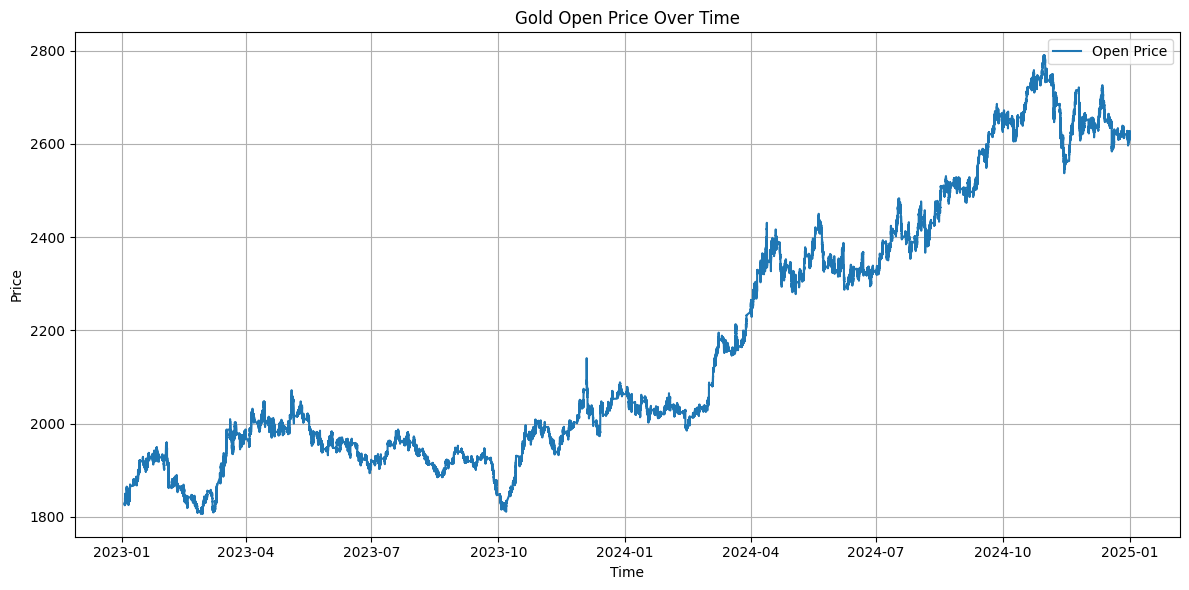
\includegraphics[width=0.8\textwidth]{Figures/Time Series Gold Price.png}
    \caption{Time Series Gold Price}
    \label{fig:time_series_goldprice}
\end{figure}

%--------------------------------------------------------------------------
% 13. August 2025

